% !TEX program = xelatex
% !TeX encoding = utf8
% !TeX spellcheck = pl-PL

%%%%%%%%%%%%%%%%%%%%%%%%%%%%%%%%%%%%%%%%%%%%%%%%%%%%%%%%%%%%%%%%%%%%%%%%%%%
% Wybierz rodzaj pracy dyplomowej oraz wydział
% Pick thesis type and faculty
%%%%%%%%%%%%%%%%%%%%%%%%%%%%%%%%%%%%%%%%%%%%%%%%%%%%%%%%%%%%%%%%%%%%%%%%%%%
\documentclass[thesis=inz,faculty=ee]{EE-dyplom} 
\usepackage{amsmath}
\usepackage{amssymb}
\usepackage{bbm,graphicx} 

    %add P.H.
    %\usepackage[default]{sourcecodepro}
    %\usepackage[T1]{fontenc}

% thesis=[inz|mgr|bsc|msc]
%  * inz - praca inżynierska
%  * mgr - praca magisterska
%  * bsc - bachelor thesis
%  * msc - master thesis

% Skróty nazw wydziałów zgodne z domenami internetowymi
% Abbreviations of Faculties according to Internet subdomains
% faculty=[
%	arch,
%	gik,
%	ee,
%	wip
%	]

%%%%%%%%%%%%%%%%%%%%%%%%%%%%%%%%%%%%%%%%%%%%%%%%%%%%%%%%%%%%%%%%%%%%%%%%%%%
% Konfiguracja - do personalizacji
% Configuration - to be personalized
%%%%%%%%%%%%%%%%%%%%%%%%%%%%%%%%%%%%%%%%%%%%%%%%%%%%%%%%%%%%%%%%%%%%%%%%%%%
 \instytut{Instytut Sterowania i Elektroniki Przemysłowej}
\kierunek{Informatyka Stosowana}
%\specjalnosc{Rzeczowidztwo}
\title{Porównanie wydajności wybranych języków programowania w realizacji sieci neuronowych do przetwarzaniu obrazów\\
}


\engtitle{Comparison of the performance of selected programming languages in the implementation of neural networks for image processing}
\album{146703}
\author{Piotr Heinzelman}
\promotor{dr inż. Witold Czajewski}
\date{2024}
\longdate{2024-09-27}

%\grantlicense{TRUE} % [TRUE|FALSE]

%%%%%%%%%%%%%%%%%%%%%%%%%%%%%%%%%%%%%%%%%%%%%%%%%%%%%%%%%%%%%%%%%%%%%%%%%%%
% Streszczenie pracy i abstract.
% In case of thesis in English swap the order - English version goes first.
%%%%%%%%%%%%%%%%%%%%%%%%%%%%%%%%%%%%%%%%%%%%%%%%%%%%%%%%%%%%%%%%%%%%%%%%%%%
\streszczeniepracy{



Idea jest taka, by sprawdzić jak w różnych językach progrmowania wygląda jakieś kompleksowe zastosowanie sieci neuronowych do przetwarzania obrazów. Dwa najpopularniejsze języki to C++ i Python, potem jest Matlab. Dość powszechne jest też uruchamianie kodu Pythona w Colabie. Chodzi o zrobienie dokładnie kilku takich samych aplikacji w kilku językach i porównanie ich pod różnymi kątami. Przykładowe aplikacje to: klasyfikacja obrazów, rozpoznawanie obiektów na obrazach, śledzenie obiektów, segmentacja obiektów, modyfikacja obrazów czy ich fragmentów.

Jeśli taki zakres projektu Panom odpowiada, to proszę dać znać, a założę dedykowany projektowi kanał na Teamsach, gdzie będziemy się dalej komunikować.

} % koniec streszczenia

\slowakluczowe{A, B, C}

\thesisabstract{
This is abstract. This one is a little too short as it should occupy the whole page.

\lipsum[1-4]
} % end of abstract

\thesiskeywords{X, Y, Z}

%%%%%%%%%%%%%%%%%%%%%%%%%%%%%%%%%%%%%%%%%%%%%%%%%%%%%%%%%%%%%%%%%%%%%%%%%%%
% Tu zaczyna się dokument
% Here is the beginning of the document
%%%%%%%%%%%%%%%%%%%%%%%%%%%%%%%%%%%%%%%%%%%%%%%%%%%%%%%%%%%%%%%%%%%%%%%%%%%
\begin{document}
    % Strony nagłówkowe
    % Headers
    \frontpages

    % Właściwa treść jest w pliku tekst/main.tex
    % Real contents is in tekst/main.tex
    % Rozdziały zaczynają się od "chapter"
\chapter{Wstęp}
% Praca podzielona na mniejsze pliki włączane za pomocą input
% Zajrzyj do pliku tekst/wstep.tex
Dobór algorytmu do zadania jest bardzo ważny, zdecydowanie ważniejszy niż dobór języka - jednak nie będzie on głównym tematem tej pracy. Tu zakładamy użycie tych samych algorytmów i porównujemy wydajności implementacji algorytmu w różnych "językach". Teoretycznie wyniki powinny być zbliżone przy założeniu, że programy doskonale wykorzystują możliwości sprzętu. Celem pracy jest porównanie, które języki ogólnego przeznaczenia liczą szybciej, które lepiej wykorzystują dodatkową infrastrukturę taką jak \textit{wątki}, \textit{procesy},  \textit{hyperThreading}, czy rdzenie \textit{CUDA} na kartach graficznych.
Jeśli gdzieś zaobserwujemy różnice - to będą one wynikały zastosowania innych języków, które w odmienny sposób zapisują i odczytują liczby, kolejkują zadania czy optymalizują wygenerowany kod. \newLine 
Jednak zanim przejdziemy do~porównania, przyjrzymy się modelom matematycznym, a z ich pomocą zbudujemy prosty model obiektowy. Następnie przetestujemy model obiektowy, prześledzimy przetwarzanie na najniższych poziomach, aż do pojedynczych operacji. Te działania pomogą nam przygotować zadania numeryczne, do rozwiązania których użyjemy maszyn cyfrowych.

\begin{lstlisting}
/*

4. Realizacje obliczeń Klasyfikowanie pisma odręcznego MLP z wykorzystaniem danych MNIST
a) Matlab
b) Python -numpy, -sklearn
c) Python -tensorflow
d) własna implementacja w Java

Cel podstawowy: porównanie wydajności realizacji w zależności od Języka.
Cele dodatkowe: potwierdzenie poprawności własnej implementacji przez porównanie wyników,


5) realizacja Klasyfikowanie pisma odręcznego sieci głębokie CNN realizacja sieci z wykorzytsniem bibliotek.
a) Matlab
b) Python tensorflow.keras
c) własna implementacja Java lub C++ libtorch

Cel podstawowy: porównanie wydajności implementacji. Zbadanie wydajności uczenia sieci.
Cele dodatkowe: potwierdzenie poprawności własnej implementacji w Java lub C++


6) Rozpoznawanie twarzy sieci głębokie CNN
a) Matlab
b) Python tensorflow.keras
c) własna implementacja Java lub C++ libtorch

Cel podstawowy: porównanie wydajności implementacji.


7) Klasyfikacji obrazów z wykorzystaniem sieci głębokiej CNN
a) Matlab
b) Python tensorflow.keras
c) C++ libtorch

Cel podstawowy: porównanie wydajności implementacji i wydajności procesu uczenia nadzorowanego.

8) detekcja i segmentacji obiektów sieci głębokiej CNN
b) Python tensorflow.keras
c) C++ libtorch

Cel podstawowy: porównanie wydajności implementacji.


*/
\end{lstlisting}


% fragment nieużywany albo jeszcze niedodany można zakomentować
\chapter{Teoria}
\input{tekst/teoria}


\chapter{Model obiektowy}

Proces przetwarzania możemy opisać i analizować jako współpracę obiektów dwu klas: neuronu (\textit{Neuron}) i warstwy (\textit{Layer}). Ujęcie obiektowe umożliwia ściślejszą hermetyzację, ułatwia realizację współbieżności przetwarzania. Realizacja w tym modelu umożliwia wykorzystanie wzorców projektowych w tym: \textit{dziedziczenia}, \textit{interfejsu} czy \textit{obserwatora}.

\section{ Obiekt klasy Layer }

\begin{figure}[h]
	\centering 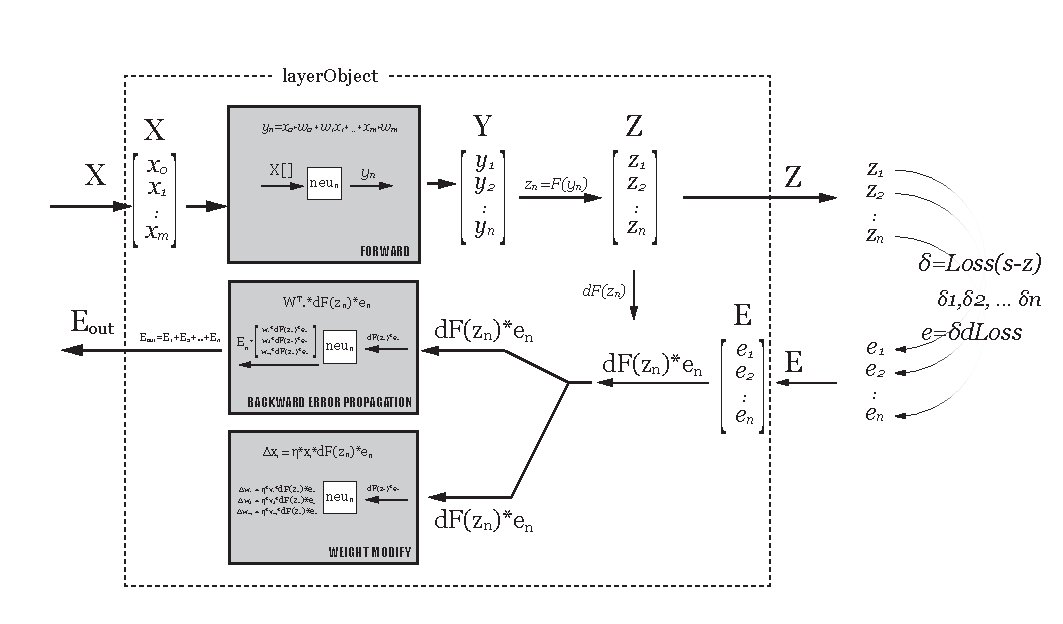
\includegraphics[width=\textwidth]{gfx/rys1_4.pdf} 
	\caption{ Przepływu sygnałów w obiekcie Layer  }
	\label{rys:modelobiektowegoneuronuszkic1}
\end{figure}

Każdy obiekt Layer ma własną kolekcję obiektów klasy Neuron. Dysponuje też polami danych np. X, które są zbiorami wartości. I tak pole danych X jest zbiorem wartości { \(x_0, x_1, ... x_m \) }. pole danych Y jest zbiorem wartości { \(y_0, y_1, ... y_m \) }. Z matematycznego punktu widzenia, można powiedzieć że wektor X jest wektorem zmiennych niezależnych X = [ \(x_0, x_1, ... x_m \) ], skoro tak, to i \textbf{pochodne składników tych wektorów będą niezależne względem siebie}. Z informatycznego punktu widzenia pole X jest zbiorem wartości  \(x_0, x_1, ... x_m \), które może być realizowane przez takie struktury danych jak \textit{zbiór}, \textit{lista}, \textit{tablica} czy \textit{wektor}. Zależnie od języka programowania pewne struktury będą wygodniejsze do wykorzystania od innych. Struktura \textit{tablica} jest najprostsza, kolejne wartości są indeksowane liczbą całkowitą, a sama tablica po utworzeniu nie może zmieniać swojego rozmiaru. 

Obiekty klasy Layer wywołuje dla wszystkich neuronów ze swojej kolekcji żądania wykonania obliczeń. Obiekty klasy Neuron mają dostęp do obiektu rodzica, a dzięki temu mają także dostęp do niektórych pól danych obiektu Layer. Neurony nie mają jednak bezpośrednich połączeń między sobą. 







\begin{figure}[h]
	\centering 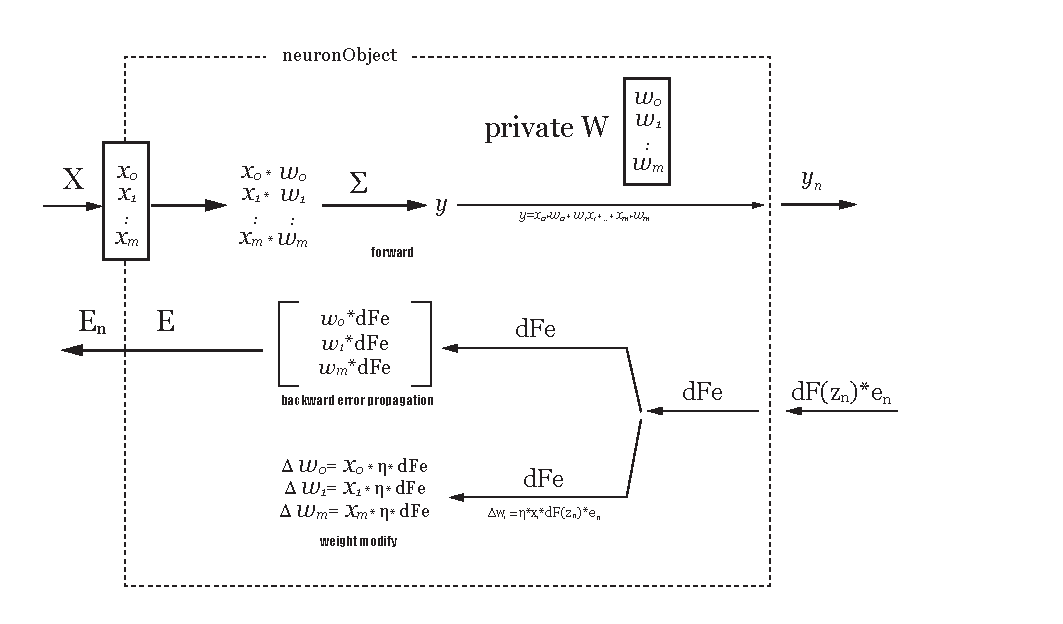
\includegraphics[width=\textwidth]{gfx/rys1_5.pdf} 
	\caption{ Przepływu sygnałów w obiekcie Neuron }
	\label{rys:modelobiektowegoneuronuszkic2}
\end{figure}

Obiekty klasy Neuron są bardzo proste i lekkie, realizują kilka operacji matematycznych wywoływanych na żądanie warstwy rodzica. Do obliczeń używają wewnętrznych zmiennych wag zorganizowanych w tablicę \( W = [ w_0, w_1, ... w_m ]\) , oraz dostarczonych przez rodzica zmiennych skalarnych oznaczanych małymi lierami np. \(\eta\), lub tablic skalarów oznaczanych dla rozróżnienia wielkimi literami np. pole X. 
 
\newpage
\begin{figure}[h]
	\centering 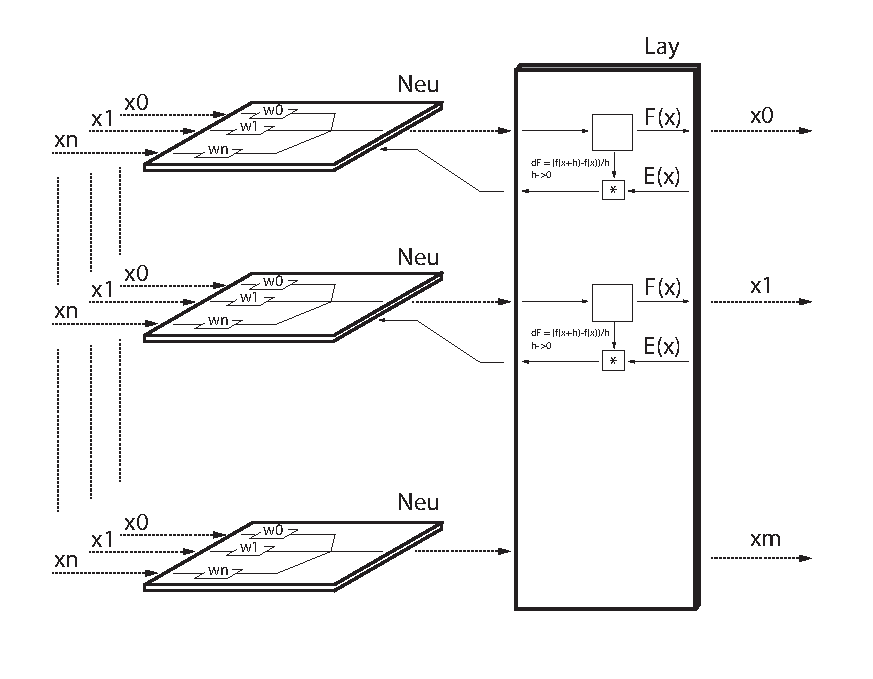
\includegraphics[width=0.5\textwidth]{gfx/3d.pdf} 
	\caption{ współpraca klas Neuron / Layer }
	\label{rys:modelobiektowegoneuronuszkic2}
\end{figure}
\section{ Propagacja sygnału pomiędzy obiektami }
Pojedynczy neuron odczytuje wartości wektora wejściowego - tablicy \(X\) o określonym rozmiarze \(m\), przekazanego przez rodzica. Oblicza iloczyn odpowiednich wag i wartości, a następnie sumuje uzyskane iloczyny. Obliczoną \textbf{wartość skalarną zmiennoprzecinkową} - zwraca jako wynik operacji.
\newline
\begin{lstlisting}
    public float forward( float[] X ) {
        float sum=0;
        for ( int m=0; m<W.length; m++ ) {
            yi= X[m]*W[m];
            sum = sum + yi;
        }
        return sum;
    }
\end{lstlisting}
obiekt Layer dla otrzymanych wartości \(y_1, y_2, ... y_n\) oblicza wielkość funkcji aktywacji \(z_i = f(y_i)\). 
Metoda wyliczająca wielkość funkcji aktywacji zależnie do rodzaju warstwy:
\begin{lstlisting}
    private float F ( float y ){
        float z;
        switch (this.lType) {
            case sigmod: { return ( 1/(1 + Math.exp( -y ))); }
            case linear:
                default: { z=y; break; }
        }
        return z;
    }
\end{lstlisting}

Wielkości te zebrane w tablicę tworzą wartość wyjściową Z. 
Przy okazji obliczamy także wartość pochodnych funkcji F w punktach \(y_i\) i zapisujemy w tablicy dFofZ).

\begin{lstlisting}
    public void forward(){
        for ( int n=0; n<neurons.length; n++ ) {
            Y[n] = neurons[n].forward( X );
            Z[n] = F ( Y[n] );
            dFofZ[n] = dF( Z[n] );
        }
    }
\end{lstlisting}

Zestawienie pochodnych funkcji straty \(Loss\) oraz funkcji aktywacji \(dF(y)\) zależnie od rodzajów warstw ~\ref{tab:funkcjeaktywacji}.

\begin{lstlisting}
    private float dF (float z ){
        float df;
        switch (lType) {
            case sigmod: { df = z*(1-z); break; }
            case linear:
            default: { df=1; break; }
        }
        return df;
    }
\end{lstlisting}


Pierwsze programy napisane przy użyciu modelu wykonują poprawnie przykładowe zadania z \cite{profWłodzimierzKasprzak2024wyklad}.






 
\chapter{Przetwarzanie numeryczne}
Z punktu widzenia matematyków różnica pomiędzy 1.0000000000000001 a 1.0 jest spora, ponieważ pomiędzy tymi wartościami mamy nieskończenie wiele liczb, natomiast przy obliczeniach, których dokonujemy używając maszyn cyfrowych musimy zważyć, czy zwiększać dokładność zwiększając ilość bitów zajmowanych przez liczby, jednocześnie zmniejszać szybkość operacji, czy wykorzystać mniej dokładne reprezentacje zyskując na szybkości pewnych operacji. 

\section{Kodowanie}
Najczęściej używaną reprezentacją liczb rzeczywistych jest opisana przez normę IEEE 754. Norma ta definiuje zapis liczby w 32, 64 liczb 128 bitach. W językach programowania dostępne jako klasy \textit{Float}, \textit{Double}. 



\begin{itemize}
    \item Matlab: przypisanie a=1.0000000000000001 //  a=1;
    \item Python: print (.000600000000000000001) // 0.0006. 
    \item Java: \(0.1 + 0.2 = 0.30000000000000004.\)
\end{itemize}

Do zastosowań specjalnych możemy użyć specjalnych formatów zapisu np. BigDecimal w Java o~większej dokładności (większej liczbie cyfr znaczących), lecz o~dużo dłuższym czasie operacji.  
\newline
Float - 0.002 [sek.] / BigDecimal 0.042 [sek.]

\break

\section{operacje równoległe}
operacje niezależne - na rysunku oznaczone kolorem zielonym - takie jak mnożenie wag przez wartości wejściowe możemy wykonywać równolegle, wykorzystując osobne wątki, procesy, rdzenie. Operacje sumowania nie są operacjami niezależnymi. 

\begin{figure}[h]
	\centering 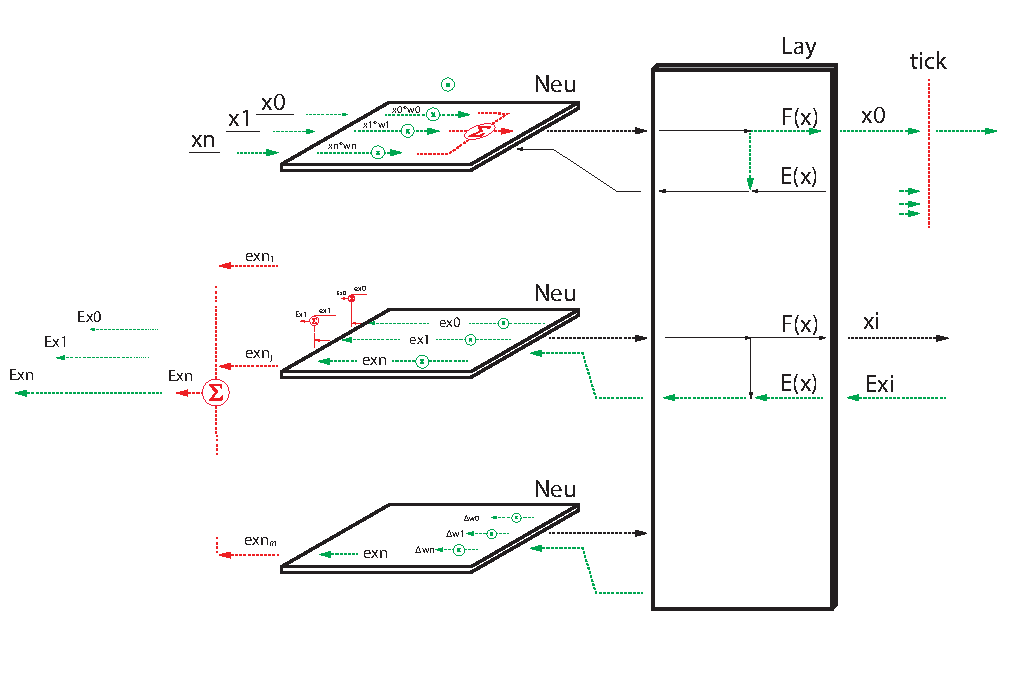
\includegraphics[width=0.9\textwidth]{gfx/3drev.pdf} 
	\caption{ operacje niezależne i operacje wymagające synchronizacji}
	\label{rys:operacjesynch}
\end{figure}


Sumowanie a+b+c+d realizowana jest analogiczne do zdegenerowanego drzewa binarnego czyli 
(((a+b)+c)+d)... nie jest operacją równoległą. Przy dużej ilości składników możemy spróbować zastosować zwykłe drzewo binarne nie zdegenerowane, a operacja dodawania może stanie się częściowo równoległa  ( (a+b)  +  (c+d) ... ).
Maszyny cyfrowe obecnie nie są wyposażone w sumatory wielokanałowe pozwalające dodawać więcej niż 2 liczby jednocześnie. Najprostsza realizacja fizyczna takiego sumatora jest możliwa do realizacji w układach FPGA, można także zastosować nawiasy.

\begin{figure}[h]
	\centering 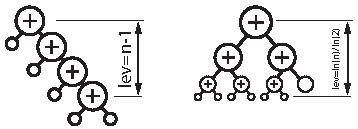
\includegraphics[width=0.7\textwidth]{gfx/sum.pdf} 
	\caption{ drzewo zdegenerowane i niezdegenerowane}
	\label{rys:operacjesynch}
\end{figure}

\break

 
\section{Dodawanie równoległe}
różnice w szybkości dodawania: (C++) 
\begin{equation*}
b=a1+a2+a3+a4+...+a1024;
\end{equation*}
czas wykonania: \textbf{0.247875 [sek.]}

\begin{equation*}
b=((..((a1+a2)+(a3+a4))+((a5+a6) ...
\end{equation*}
czas wykonania: \textbf{0.09568 [sek.]} 
\newline 
\newline Ponad dwukrotne zwiększenie szybkości przez dodanie nawiasów. 
przy 32 składnikach mamy 16 + 8 + 4 + 2 + 1 dodawań, jednak pierwsze 16 może być wykonane równolegle, kolejna 8 także jest od siebie niezależna, podobnie 4 i 2. Czyli dla 32 elementów  mamy 31 dodawań w 5 poziomach. Dla 1024 składników mamy 1023 dodawania, 512+256+128...+1 w 10 poziomach. Podsumowując 1023 dodawania możemy wykonać w czasie takim jak 10 dodawań korzystając z osobnych 512 rdzeni CUDA zakładając że dostęp do pamięci będzie niezależny. Korzystając ze zwykłego CPU poszczególne rdzenie będą czekały się w kolejce po odczyt wartości składników oraz w drugiej kolejce do zapisu wyników w pamięci. Jeśli kod będzie "optymalizowany" np. przez procesor i zmieni się kolejność niektórych działań, wynik sumowania może być nieprawidłowy.

\section{ Wątki }
Rozdzielenie przetwarzania w ramach procesu na wątki umożliwia równoległe przetwarzanie danych i jest wspierane przez nowoczesne procesory. Proces będzie miał do dyspozycji kilka niezależnych jednostek liczących ALU, więc niezależne operacje będą wykonywane w tym samym czasie. A zatem pojedyncze mnożenie zajmie tyle czasu co kilka mnożeń na kilku rdzeniach. 

\section{ HyperWątki HT}
Technologia wprowadzone przez Inter HyperThread(R) tworzy dwie kolejki rozkazów dla jednego rdzenia, co dla systemu operacyjnego wygląda na dwa niezależne rdzenie. W rezultacie w czasie gdy jedna kolejka wykorzystuje jednostkę liczącą, w drugiej kolejce może być bez przeszkód wykonana instrukcja odczytania lub zapisu danych do pamięci - a te instrukcje zajmują nawet kilkanaście cykli zegara. W tej sytuacji mamy zwiększone wykorzystanie potencjału pojedynczego rdzenia. 

\section{ Pamięć operacyjna }
Ponieważ dostęp do \textit{magistrali pamięci} jest synchroniczny, to nawet jeśli samo przetwarzanie przez ALU będzie równoległe, to odczyt i zapis w pamięci będzie miał charakter zbliżony do synchronicznego. Nawet przy dwu niezależnych kanałach po 128 bitów w każdym (DDR5). 

\section{ Rdzenie CUDA }
Procesory ogólnego przeznaczenia, mimo wielu wysiłków, nie są w stanie zapewnić w pełni równoległego przetwarzania. Równoległe przetwarzanie mogą zapewnić np. procesory graficzne, w których znajduje się wiele jednostek obliczeniowych, ale przede wszystkim dostęp do pamięci jest rzeczywiście równoległy. Procesory graficzne projektowane były do obliczeń translacji punktów w przestrzeni, a operacje te sprowadzały się do mnożenia macierzy współrzędnych znormalizowanych punktu przez macierz translacji:

\begin{equation*}
  T =  \begin{bmatrix}
 1 & 0 & 0 & x\\
 0 & 1 & 0 & y\\
 0 & 0 & 1 & z\\
 0 & 0 & 0 & 1
        \end{bmatrix} ,
  O_x =  \begin{bmatrix}
 1 & 0 & 0 & 0\\
 0 & c & -s & 0\\
 0 & s & c & 0\\
 0 & 0 & 0 & 1
        \end{bmatrix} ,
R =  \begin{bmatrix}
 1 & 0 & 0 & 0\\
 0 & 1 & 0 & 0\\
 0 & 0 & 1 & 0\\
 0 & 0 & 1/d & 0
        \end{bmatrix} 
\end{equation*}

a po rozpisaniu mamy:
\begin{equation*}
\begin{matrix}
  X - x*m[0][0] + y*m[1][0]+z*m[2][0] + w*m[3][0] \\

  Y - x*m[0][1] + y*m[1][1]+z*m[2][1] + w*m[3][1] \\

  Z - x*m[0][2] + y*m[1][2]+z*m[2][2] + w*m[3][2] \\

  W - x*m[0][3] + y*m[1][3]+z*m[2][3] + w*m[3][3]  \\
  \end{matrix}
\end{equation*}

i są to te same obliczenia, które wykonujemy wielokrotnie podczas pracy z matematycznymi modelami sieci neuronowych:
\begin{equation*}
  y - x_0*w_0 + x_1*w_1 +x_2*w_2 ... +x_2*w_2;
\end{equation*}
a jeśli będą one wykonane przez osobne rdzenie CUDA, a wyniki będą zapisane w pamięci VRam o dostępnie równoległym - wtedy wiele takich operacji zajmie dokładnie tyle samo czasu co pojedyncza operacja. Idealnie byłoby gdyby cała praca odbywała się w VRAM i na rdzeniach CUDA bez konieczności przesyłania danych w każdym cyklu do pamięci operacyjnej RAM. Jeśli zbiór danych w całości znajdowałby się w VRAM, to przejście sygnałów przez jedną warstwę sieci trwałoby tyle co jedna operacja, a propagacja przez sieć trwałaby tyle razy dłużej ile warstw mamy w sieci. Powrót sygnału w postaci wielkości błędu podobnie zajmowałby mniej więcej tyle czasu. (O ile operacje mnożenia możemy wykonać równolegle to operacje wielokrotnego dodawania już nie do końca). 
Równoległe zmiany kilku wag również byłyby dokonywane w takim czasie jak zmiana pojedynczej wagi.
\newline
Wprowadzanie na rynek gier sieciowych wymagających do zabawy coraz wydajniejszych kart graficznych oraz pojawienie się wirtualnych walut typu Bitcoin wydobywanych - obliczanych właśnie przy użyciu takiego sprzętu zwiększyła zapotrzebowanie na coraz wydajniejsze jednostki mimo sporych kosztów jak dla użytkownika indywidualnego. 
\newline
Dostępność cenowa coraz wydajniejszych jednostek, które przyspieszają obliczenia nawet o kilka rzędów wielkości, spowodowała, że budowanie prawdziwie używalnych modeli stało się możliwe. A temat \textit{„sztucznej inteligencji”} znany wcześniej jedynie garstce naukowców, stał się nagle tematem bardzo popularnym. 

\section{Matlab}
Dodatek Parallel computing w Matlab umożliwia wykonywanie obliczeń równolegle, w osobnych wątkach, procesach a także z wykorzystaniem kart graficznych (obecnie tylko NVidia). Dodatki Optimalization Toolbox i Optimalization Computing Toolbox optymalizują tworzony kod zwiększając jego wydajność. Dodatek Deep Learning Toolbox dostarcza gotowych metod do obliczeń sieci neuronowych.

\section{Python}
Metody do obliczeń sieci neuronowych w języka Python dostarczone są w bibliotekach scikit-learn i TensorFlow2 a dostarczają one gotowych metod przydatnych w obliczeniach sieci neuronowych. Wykorzystują one możliwości równoległego przetwarzania, które oferuje sprzęt na którym uruchamiany jest kod.

https://www.geeksforgeeks.org/matplotlib-tutorial/
matlabplotlib 

%\chapter{Zagadnienia}
%\input{tekst/zagadnienia}

\chapter{Jednowymiarowa regresja liniowa}

\section{Wprowadzenie}
Przykłady obliczeń Python i Matlab zostały zaczerpnięte z \cite{ossowski2023}.
\textbf{Pełen kod dostępny na github:} https://github.com/piotrHeinzelman/inz/tree/main/MixedProj/01.polyfit
w przypadku Matlab i Python korzystam z dostępnych funkcji, w przypadku Java obliczam wg. wzoru ~\ref{eq:linearregresion}. Obliczenia różnymi metodami dają zbliżone wyniki, więc zakładam że moje implementacje są poprawne. 

 
W pracy tam gdzie możliwe staram się wykorzystać dostarczone funkcje liczące. I tak dla Matlab i dla Python wykorzystałem zaimplementowaną funkcję "polyfit". W kodzie Java musiałem sam zaimplementować funkcję liczącą dla porównania wydajności. W programach nie porównuję czasu ładowania i przygotowania danych ponieważ chcę wykonywać obliczenia dla tych samych wartości czytanych z tych samych plików, natomiast nie jest moim celem optymalizacja wczytywania danych z pliku.

\newpage
\section{Prowadzenie badania}
Programy w kolejnych językach uruchamiam poniższym kodem:

\begin{lstlisting}[ basicstyle=\tiny]
./matRun >> output.txt
./pyRun  >> output.txt
./javaRun >> output.txt

//matRun
echo "--- Matlab app start: ---"
/usr/local/MATLAB/R2024a/bin/matlab  -nodisplay -nosplash -nodesktop -batch 'run matlab.m'

//pyRun
echo "--- Python app start: --- "
python main.py

// javaRun
javac Main.java 
echo "--- Java app start: ---"
java Main
\end{lstlisting}


\section{Kod realizujący obliczenia}


\begin{lstlisting}[ basicstyle=\tiny]
//                  --- MATLAB ---

    a = polyfit(x,y,1);

//                  --- Python --- 

    a = np.polyfit(x,y,1)

//                  ---  Java --- 

     for (int i = 0; i < x.length; i++) {
            xsr += x[i];
            ysr += y[i];
        }
        xsr = xsr / x.length;
        ysr = ysr / y.length;

        for (int i = 0; i < x.length; i++) {
            sumTop += ((x[i] - xsr) * (y[i] - ysr));
            sumBottom += ((x[i] - xsr) * (x[i] - xsr));
        }
        w1 = sumTop / sumBottom;
        w0 = ysr - w1 * xsr;

//               --- C++ ---

      for ( int i=0; i<len; i++ ){
         xsr +=  X[i];
         ysr +=  Y[i];
      }
   xsr=xsr / len; ysr=ysr / len;
   double sumTop=0.0;
   double sumBottom=0.0;

      for ( int i=0;i<len;i++ ){ //  xtmp = X[i]-sr ! ;
       sumTop   += ((X[i]-xsr)*(Y[i]-ysr));
      sumBottom += ((X[i]-xsr)*(X[i]-xsr));
      }
      w1 = sumTop / sumBottom;
      w0 = ysr -(w1 * xsr) ;
        
.   
\end{lstlisting}

\newpage
\section{Uzyskane wyniki}

\begin{figure}[h]
    	\centering 
            \includegraphics[width=0.70\linewidth]{gfx/fig01.pdf} 
\end{figure} 
\begin{figure}[h]
    \begin{subfigure}{.5\textwidth}
    	\centering 
            \includegraphics[width=0.95\linewidth]{gfx/01a.png} 
    \end{subfigure} %
    \begin{subfigure} {.5\textwidth}
    	\centering 
            \includegraphics[width=0.95\linewidth]{gfx/fig01_PC2.pdf} 
    \end{subfigure} 
    \caption{Porównanie czasów obliczania regresji liniowej}
\end{figure} 

\chapter{Klasyfikowanie pisma odręcznego MLP}
\section{Wstęp}
Porównuję dokładność sieci rodzaju MLP w zależności od ilości danych - 
podczas uczenia sieci wycinkiem danych uczących, dokładność sieci wzrasta do granicznej 88,34\% przy wykorzystaniu pełnego zestawy danych uczących.
Zmiana ilości neuronów w dwu warstwach również wpływa na dokładność sieci i jest największa przy 64 neuronach. Zwiększenie lub zmniejszenie liczby neuronów zmniejsza dokładność sieci. Długość procesu uczenia wynosiła 5000 epok. Szacowanie przeprowadzałem w języku Matlab. Metodę uczenia wybrałem metodę największego spadku, ponieważ przy wyborze metody LM miałem za mało pamięci dla takiej konfiguracji sieci. (wymagane 21Gb)


\begin{figure}[h]
    \begin{subfigure}{.5\textwidth}
    	\centering 
            \includegraphics[width=0.90\linewidth]{gfx/fig03b.pdf} 
    \end{subfigure} %
    \begin{subfigure} {.5\textwidth}
    	\centering 
            \includegraphics[width=0.90\linewidth]{gfx/fig03a.pdf} 
    \end{subfigure} 
    \caption{Szacowanie parametrów sieci}
\end{figure} 

Porównanie czasów wykonania uczenia 64 neuronów w 2 warstwach i 5000 epok dla różnych języków. 
Dla Matlab wyniki uzyskane w systemie operacyjnym Windows 10 oraz Arch Linux w trybie tekstowym, dodatkowo wyniki przy obliczeniach domyślnych proponowanych przez program, w porównaniu z wymuszeniem obliczeń tylko na GPU. Dość zaskakująca jest różnica w szybkości obliczeń na GPU w zależności od platformy. Odpowiednio w systemie Windows 10 obliczenia trwają 419-425 sek., Linux Arch wykona te obliczenia w czasie 205-211 sek. 
\section{Dane treningowe}
Dane treningowe i testowe - zestaw pisanych ręcznie cyfr - pochodzą z zasobów MNIST (yann.lecun.com). w kodzie Java dodałem zestaw metod umożliwiający m.in. podejrzenie wektorów treningowych jako obrazy, zapisanie wag warstwy jako obraz, i inne.

\begin{figure}[h]
	\centering \includegraphics[width=0.9\textwidth]{gfx/mnist_prev.png} 
	\caption{ podgląd próbki wektorów uczących}
	\label{rys:podglad_mnist}
\end{figure}

poniżej kod ładujący dane, oraz metody narzędziowe:

\begin{lstlisting}[ basicstyle=\tiny]

public  void prepareData( int percent ){
   trainYfile =  loadBin( "../data/" + "t10k-images-idx3-ubyte", 8, percent*600 ); //offset=8, size=percent*600  // OK
   testYfile =  loadBin( "../data/" + "t10k-labels-idx1-ubyte",  8, percent*100 ); // offset=8, size=percent*100 // OK

   trainY = new float[percent*600][];
   testY  = new float[percent*100][];
   //train Y
   for (int i=0;i<percent*600;i++){
      trainY[i] = new float[]{ 0.0f, 0.0f, 0.0f, 0.0f, 0.0f, 0.0f, 0.0f, 0.0f, 0.0f, 0.0f };
      trainY[i][ trainYfile[i] ]=1.0f;
   }

   byte[] trainXfile = loadBin(path + trainXname, 16, percent * 784 * 600);// offset=16 size=percent*784*600
      trainX=new float[percent*600][784];
         for (int i=0;i<percent*100;i++) {
            int off=i*784;
            for (int j=0;j<784;j++){
               trainX[i][j]=Byte.toUnsignedInt( trainXfile[off+j] )/16; 
               
        }}} catch (IOException e) { throw new RuntimeException(e); }
   }


    public static byte[] loadBin( String filename, int offset, int len ) throws IOException {
        byte[] bytesBuf = new byte[ len ];
        File f = new File( filename );
        FileInputStream fis = new FileInputStream( filename );
        fis.skip(offset);
        fis.read( bytesBuf, 0, len );
        return bytesBuf;
    }

    public static float[] vectorSubstSsubZ( float[] s, float[] z ){
        float[] out = new float[ z.length];
        for ( int i=0;i<z.length; i++ ){
            out[i] = ( s[i] - z[i] );
        }
        return out;
    }

    public static float meanSquareError( float[] s, float[]z ){
        float out = 0.0f;
        for ( int i=0;i<z.length; i++ ){
            float delta = s[i] - z[i];
            out+=delta*delta;
        }
        return out;
    }
 
    public static BufferedImage arrayOfFloatToImage( float[] data , int xScale ){
        int width = data.length/xScale;
        int height = 510;
        float min = data[0];
        float max = data[0];
        for ( int i=1;i< data.length;i++ ){
            if ( data[i]<min ) { min=data[i]; }
            if ( data[i]>max ) { max=data[i]; }
        }
        float delta=( max-min )/(height-10);
        BufferedImage image = new BufferedImage( width , height , TYPE_INT_RGB );

        int pointColor = (255*255*240)+(255*244)+244;
        for ( int i=0;i<width;i++ ){
            int val=(int) (( data[xScale*i]-min )/delta ) ;
            image.setRGB( i, 5+val , pointColor );
        }
        return image;
    }

    public static void saveImg( BufferedImage image, String nameSuffix ){
        File file = new File("image"+nameSuffix+".png");
        try {
            ImageIO.write(image ,  "png", file );
        } catch (IOException e) {
            throw new RuntimeException(e);
        }
    }
}
\end{lstlisting}

\section{Uzyskane wyniki}
\begin{figure}[h]
    	\centering 
            \includegraphics[width=0.88\linewidth]{gfx/fig03.pdf} 
\end{figure} 


\newpage
\section{Kod realizujący obliczenia}

Matlab:
\begin{lstlisting}

    net = feedforwardnet([ 64, 64 ],'traingd'); 
    net.trainParam.epochs = 5000;
    net.trainParam.goal   = 0.03;
    net.input.processFcns = {'mapminmax'};  

    gxtrain = gpuArray( xtrain );
    gytrain = gpuArray( ytrain );

    ST = datetime('now');

    gpu=true;
    if ( gpu )
        %GPU
        net = configure(net,xtrain,ytrain);
        net = train(net, gxtrain, gytrain,'useParallel','yes','useGPU','yes');
    else
        %No GPU
        net = train( net, xtrain, ytrain );
    end    
    
    ED = datetime('now');

    z = net( xtest );
    flatZ = aryOfVectorToAryOfInt( z );
    flatZtest = aryOfVectorToAryOfInt( ytest ); 
    accuracy = accuracyCheck(flatZ, flatZtest);

    D = duration( ED-ST );

    fprintf('# MLP: 2x64Neu * 5000 cycles:\n' );
    fprintf( '# accuracy: a:%f\n\n' , accuracy );
    fprintf ('m[]=%f\n' , seconds(D)  );

\end{lstlisting}

\newpage
\section{Własna implementacja w Java}
Do napisania programu użyłem własnego, opisanego we wcześniejszych rozdziałach modelu obiektowego sieci neuronowych. Sieć ta pracuje dużo wolniej niż rozwiązanie w matlab, uczenie sieci zajmuje aż 14400 sek. Najważniejszym celem napisania tego programu było sprawdzenie czy sieć oparta na modelu obiektowym działa, i czy osiągnie podobny poziom dokładności jak gotowe rozwiązanie z Matlab. Okazuje się, że podobnie jak sieć w Matlab, ta napisana w Java osiąga dokładność około 87\%;
Kod celowo nie jest optymalizowany pod kątem wydajności  - chodziło mi o łatwość czytania i zrozumienia modelu, a także potwierdzenie że sieć oparta na tym modelu uczy się podobnie jak gotowe rozwiązanie z Matlab. W kodzie umieściłem metody dzięki którym mogłem sprawdzić czy dane wczytują się prawidłowo. Poniżej zamieszczam kod rozwiązania:
\begin{lstlisting} [ basicstyle=\tiny]
// main.java
private float[][] testX; private float[][] testY; private float[][] trainX; private float[][] trainY;

private Layer layer1; private Layer layer2; private Layer layer3;

private Tools tools = new Tools();
int numOfEpoch=500;
float[] CSBin_data=new float[numOfEpoch];

public void prepare() {
    tools.prepareData( 100 );
    testX = tools.getTestX();
    testY = tools.getTestY();
    trainX = tools.getTrainX();
    trainY = tools.getTrainY();

    layer1=new Layer( LType.sigmod , 64 ,784 ); layer1.setName("Layer1"); // n neurons
    layer2=new Layer( LType.sigmod , 64 ,64 ); layer2.setName("Layer2"); // n neurons
    layer3=new Layer( LType.softmaxMultiClass , 10 ,64 ); layer3.setName("Layer3"); // n neurons
    layer1.rnd();  layer2.rnd();  layer3.rnd();
}

public void run() {

float Loss = 0.0f;
for (int epoch = 0; epoch < numOfEpoch; epoch++) {
    for ( int index = 0; index < trainX.length; index++ ) {
        layer1.setX( trainX[ index ] );
        layer1.nForward();
        layer2.setX( layer1.getZ() );
        layer2.nForward();
        layer3.setX( layer2.getZ() );
        layer3.nForward();

        float[] S_Z = tools.vectorSubstSsubZ( trainY[ ind_ex ], layer3.getZ() );
        layer3.nBackward( S_Z );
        layer2.nBackward( layer3.getEout() );
        layer1.nBackward( layer2.getEout() );
    }
}
        // check accuracy
int len = testX.length;
int accuracy = 0;
for (int i = 0; i < len; i++) {
    layer1.setX( testX[i] );
    layer1.nForward();
    layer2.setX( layer1.getZ() );
    layer2.nForward();
    layer3.setX( layer2.getZ() );
    layer3.nForward();

    int netClassId = tools.getIndexMaxFloat( layer3.getZ() );
    int fileClassId = tools.getIndexMaxFloat( testY[i] );
    if (fileClassId == netClassId) { accuracy++; }
    }
System.out.println(100.0f * accuracy / len + "%");
}}\end{lstlisting}

\begin{lstlisting} [ basicstyle=\tiny]
// neuron.java
public class Layer {
    private String name;
    private  LType lType;
    private  Neuron[] neurons;
    private  float X[];
    private  float Y[];
    private  float Z[];
    private  float dFofZ[];
    private  float Eout[]; // S-Z for last

    public Layer( LType lType, int n, int m ) {// n - number of neurons & output size Y[n], Z[n]
        this.lType=lType;                      // m - number of inputs  = input  size X[m]
        this.neurons = new Neuron[n];
        for (int i=0; i<n; i++){
            this.neurons[i]=new Neuron(m, this);
        }
        X = new float[m];
        Y = new float[n];
        Z = new float[n];
        dFofZ = new float[n];
        Eout = new float[m];
    }

    public void setWmn( int n, int m, float wji ){ neurons[n].setWm( m, wji ); }

    public void rnd(){
        Random random=new Random();
        for ( Neuron neu : neurons ) {
            for ( int m=0; m<X.length; m++ ) {
                neu.setWm( m , (float)( -1.0f+2.0f*random.nextFloat() )  );
            }
        }
    }

    public float[] nForward() {
        switch (lType) {
            case sigmod:
            case sigmod_CrossEntropy_Binary:{
                for (int n = 0; n < neurons.length; n++) {
                    Y[n] = neurons[n].Forward(X);
                    Z[n] = F(Y[n]);
                    dFofZ[n] = dF(Z[n]);
                }
                for (int m=0;m<Eout.length;m++){ Eout[m]=0; }
                return Z;
            }
            case softmaxMultiClass: {
                int len = neurons.length;
                float sum = 0.0f;
                float max = Y[0] = neurons[0].Forward(X);
                for (int i=1;i<len;i++){
                    dFofZ[i] = 1;
                    Y[i]=neurons[i].Forward(X);
                    if (Y[i]>max) { max=Y[i]; }
                }
                for (int i = 0; i < len; i++) {
                    Y[i] = (float) Math.exp( Y[i]-max );
                    sum += Y[i];
                }
                for (int i = 0; i < len; i++) {
                    Z[i] = Y[i] / sum;
                }
                return Z;
            }
            default: { return Z; }
        }
    }

    public void nBackward( float[] Ein ){ // S-Z or Ein
        for ( int i=0;i<neurons.length;i++ ){ Eout[i]=0.0f; }
        for ( int n=0; n< neurons.length; n++ ){
            neurons[n].Backward( Ein[n] * dFofZ[n] );
        }
    }




    private float F ( float y ){
        float z;
        switch (this.lType) {
            case sigmod:
            case sigmod_CrossEntropy_Binary:
                { z = (float) (1.0f/(1.0f + Math.exp( -y ))); break; }
            case linear:
                default: { z=y; break; }
        }
        return z;
    }

    private float dF ( float z ){
        float df;
        switch (lType) {
            case sigmod:
                { df = z*(1-z); break; }
            case linear:
            case sigmod_CrossEntropy_Binary:
            default: { df=1; break; }
        }
        return df;
    }

    // getters / setters
    public void setX( float[] _x ) {
        for ( int m=0; m<X.length; m++ ){
            this.X[m] = _x[m];
        }
    }
    public float[] getZ() { return Z; }
    public float[] getX() { return X; }
    public float[] getEout() { return Eout; }
}\end{lstlisting}

\begin{lstlisting} [ basicstyle=\tiny]
// neuron.java
public class Neuron {
    private float bias=0;
    private final float[] W;
    private final Layer parent;
    private final static float mu=0.001f;

    public void setBias( float b ) { this.bias=b; }
    public float getBias(){ return bias; }

    public Neuron( int m, Layer parent ) {
        this.parent=parent;
        this.W = new float[m];
    }

    public void setWm( int m, float wji ){
        W[m] = wji; 
    }

    public float Forward( float[] X ) {
        float res=bias;
        for ( int m=0; m<W.length; m++ ) {
            res+= X[m]*W[m];
        }
        return res;
    }

    public void Backward( float en_x_dFIznI ) {
        float[] X = parent.getX();
        for ( int m=0; m<W.length; m++ ) {
            parent.getEout()[m] += ( W[m] * en_x_dFIznI );
            W[m] += mu * en_x_dFIznI * X[m];
        }
    }
}
\end{lstlisting}

\section{Pyton}
Python -numpy, -sklearn
\begin{lstlisting}
   ?
\end{lstlisting}

c) Python -tensorflow
\begin{lstlisting}
   ?
\end{lstlisting}










\chapter{Sieci głębokie}

\chapter{Sieci głębokie}
Za protoplastę sieci głębokich można uznać zdefiniowany na początku lat dziewięćdziesiątych wielowarstwowy \textbf{neocognitron} Fukushimy, Prawdziwy rozwój tych sieci zawdzięczamy jednak profesorowi LeCun, który zdefiniował podstawową strukturę i algorytm uczący specjalizowanej \textbf{sieci konwolucyjnej} \textit{Convolutional Neural Network} skracanej tradycyjnie do CNN \cite{ossowski2023}. 

\begin{figure}[h]
    	\centering 
            \includegraphics[width=0.70\linewidth]{gfx/scan01.pdf} 
\end{figure} 

\section{CNN}
\begin{lstlisting}
https://www.mathworks.com/matlabcentral/fileexchange/74760-image-classification-using-cnn-with-multi-input-cnn?s_tid=srchtitle_support_results_1_CNN
\end{lstlisting}

\section{Python TensFlow}
..
// derative of convolution \\

https://www.physicsforums.com/threads/how-do-you-derive-the-derivative-of-a-convolution.403002/

https://dsp.stackexchange.com/questions/46746/how-to-evaluate-derivative-of-convolution-integral

https://en.wikipedia.org/wiki/Convolution


\chapter{Podsumowanie}
\label{ch:podsumowanie}

W tej zostaną opisane wyniki, oraz przesłanki, które mogą być pomocne przy doborze języka w celu realizacji głębokich sieci neuronowych w zależności od konkretnych wymagań i możliwości stawianych projektowanym rozwiązaniom.




    % Bibliografia - musi być
    % Bibliography - must exist
    \bibliografia

    % Strony końcowe - można zakomentować, jeśli zbędne
    % Additional pages - comment out if not needed
    
    % Wykaz symboli i skrótów - patrz opis w tekście przykładowym
%    \acronymslist
    % Spis rysunków
    \listoffigures
    % Spis tabel
    \listoftables
    % Załączniki (plik appendices.tex)
    \easyappendices
\end{document}
%%%%%%%%%%%%%%%%%%%%%%%%%%%%%%%%%%%%%%%%%%%%%%%%%%%%%%%%%%%%%%%%%%%%%%%%%%%

